% =====================================================================
% PeriDefT — short / journal-letter version (target ~12 pages)
% Companion to main.tex (long, 23 pages); same figures, same refs.bib.
%
% Build:
%   cd paper && pdflatex main_short && bibtex main_short \
%             && pdflatex main_short && pdflatex main_short
% =====================================================================
\documentclass[11pt,a4paper]{article}

\usepackage[T1]{fontenc}
\usepackage[utf8]{inputenc}
\usepackage{lmodern}
\usepackage{amsmath,amssymb}
\usepackage{graphicx}
\usepackage[margin=0.95in,top=0.85in,bottom=0.95in]{geometry}
\usepackage{booktabs}
\usepackage{caption}
\usepackage[hidelinks]{hyperref}
\usepackage{xcolor}
\usepackage{cite}
\usepackage{enumitem}

% Tighter caption style
\captionsetup{font=small, labelfont=bf, justification=justified, singlelinecheck=false}

% Tighter list spacing
\setlist{itemsep=2pt, topsep=3pt, parsep=0pt}

\graphicspath{{figures/}}

\title{\textbf{PeriDefT: a periodic-Fourier Transformer for 2D defect
formation energy, validated by prospective first-principles DFT}}

\author{%
  Yiming Hua, Leyan Wu, Jiaqi Bi, Sheng Chang\textsuperscript{*} \\[2pt]
  \small School of Physics and Technology, Wuhan University, Wuhan 430072, China \\[1pt]
  \small \textsuperscript{*}Corresponding author: \texttt{changsheng@whu.edu.cn}
}

\date{\today}

\newcommand{\Ef}{$E_{\mathrm{f}}$}
\newcommand{\eV}{\,\textrm{eV}}
\newcommand{\modelname}{\textsc{PeriDefT}}

\begin{document}
\maketitle

% =====================================================================
\begin{abstract}
\noindent
Most published machine-learning surrogates for 2D defect formation
energy \Ef\ are benchmarked exclusively on a held-out test fold of
the same database used for training, an evaluation that overstates
deployment utility because the chemistry of practical interest is
out of distribution by construction. We address this gap with three
coupled contributions. \emph{First}, we introduce \modelname, a
0.75\,M-parameter hybrid GNN--Transformer that augments
self-attention with a translation-invariant \emph{Periodic Fourier
Bias} (PFA) on minimum-image fractional displacements; PFA's exact
lattice-translation invariance enables stable joint training across
four DFT databases (IMP2D + JARVIS-2D + JARVIS-3D + JARVIS DFT-3D,
26\,837 samples) through per-source readout heads. \modelname\
achieves a 4-seed IMP2D test MAE of $0.486\pm0.025$\,eV ---
competitive with ALIGNN (4.03\,M, 0.540\,eV) at $1/5$ the parameter
budget --- and a 6-seed temperature-calibrated ensemble of 0.443\,eV
with 90\,\% interval coverage 93.4\,\%. \emph{Second}, we run
\textbf{60 first-principles PBE-DFT calculations} on the model's
own out-of-distribution predictions, split into a low-$E_f$
``discovery'' bucket and a high-$\sigma$ ``stress-test'' bucket.
On 37 SCF-converged candidates, the overall predicted--DFT
Pearson correlation is $+0.354$ (95\,\% bootstrap CI
$[+0.06, +0.70]$, excludes zero), and \textbf{14/20 = 70\,\%
of bucket-A picks are DFT-confirmed at $E_f<+1$\,eV}
(95\,\% CI $[50\%, 90\%]$); within bucket B,
Pearson($\sigma_{\mathrm{cal}}$, $|\mathrm{error}|$) $= -0.288$
(95\,\% CI $[-0.60, +0.09]$), suggesting $\sigma_{\mathrm{cal}}$
is informative as an in-vs-OOD bucket gate but not as a sample-level
reliability score on OOD. \emph{Third}, we release the full
pipeline (4-seed and 6-seed ensembles, 287 candidate generation,
60-candidate selection record, 125 Quantum-ESPRESSO SCF outputs)
to enable direct reuse for downstream 2D defect screening.
\end{abstract}

\bigskip
\noindent\textbf{Keywords:} 2D materials, defect formation energy,
periodic Fourier bias, multi-source training, calibrated uncertainty,
prospective DFT validation.

% =====================================================================
\section{Introduction}\label{sec:intro}

The defect formation energy
\begin{equation}
E_{\mathrm{f}}(D, q) = E_{\mathrm{tot}}(D, q) - E_{\mathrm{tot}}(\mathrm{host})
- \sum_i n_i\,\mu_i + q\,(E_F + E_{\mathrm{VBM}}) + E_{\mathrm{corr}}
\label{eq:Ef}
\end{equation}
is the central thermodynamic quantity for defect engineering in
two-dimensional materials, but a single first-principles
calculation costs tens to hundreds of CPU-hours, prohibitive for
high-throughput screening. Existing graph neural networks
(CGCNN~\cite{Xie2018CGCNN}, SchNet~\cite{Schutt2018SchNet},
ALIGNN~\cite{Choudhary2021ALIGNN}, M3GNet~\cite{Chen2022M3GNet})
and Transformer extensions (Matformer~\cite{Yan2022Matformer},
Crystalformer~\cite{Taniai2024Crystalformer},
PotNet~\cite{Lin2023PotNet}) reduce this cost by orders of magnitude,
but for point defects in 2D the published benchmarks all report
held-out-test-fold MAE on the same database used for training. This
evaluation says little about the model's deployment utility on
out-of-distribution chemistry, which is by construction what every
discovery loop encounters.

\paragraph{Contributions.}
\begin{enumerate}
\item We introduce \textbf{\modelname}, a 0.75\,M-parameter hybrid
GNN--Transformer whose self-attention carries a Periodic Fourier
Bias (PFA) that is exactly invariant under lattice translations. The
exact invariance is what makes the encoder safe to share across
geometrically heterogeneous DFT databases via per-source readout
heads (IMP2D + JARVIS-2D + JARVIS-3D + JARVIS DFT-3D, 26\,837 samples,
$3.15\times$ IMP2D). The 4-seed multi-source \modelname\ achieves
test MAE $0.486\pm0.025$\,eV, an 11\,\% improvement over a matched
single-source baseline; a 6-seed temperature-scaled ensemble reaches
0.443\,eV with 90\,\% interval coverage 93.4\,\%.

\item We report the first \textbf{prospective DFT validation} of
an IMP2D-trained 2D-defect $E_f$ model with calibrated uncertainty:
60 PBE-DFT calculations on the model's own OOD predictions, split
into a top-$\mu$ ``discovery'' bucket (n=30) and a top-$\sigma_{\rm
cal}$ ``stress-test'' bucket (n=30). On the 37 SCF-converged
candidates, \textbf{14/20 = 70\%} of bucket-A picks are DFT-confirmed
at $E_f<+1$\,eV (95\,\% CI $[50\%,90\%]$); within bucket B,
Pearson$(\sigma_{\rm cal}, |\mathrm{err}|) = -0.288$
(95\,\% CI $[-0.60, +0.09]$).

\item We release \textbf{open infrastructure}: the trained
\modelname\ ensembles, leak-free augmentation contracts (with a
self-caught-and-fixed augmentation leak, see App.~\ref{app:short_leak}),
the 287-candidate generation script, the 60-candidate selection
record, and 125 Quantum-ESPRESSO SCF outputs.
\end{enumerate}

A single-source ablation (Sec.~\ref{sec:phase1_short}) shows that
PFA, multi-scale distance bias, and a dual-stream pristine--defect
architecture are all statistically tied with the baseline at
$N_{\rm train}=8\,512$, consistent with the empirical scaling law
$\log\,\mathrm{MAE} \approx 3.39 - 0.40\log N_{\rm train} -
0.01\log N_{\rm params}$ ($R^2=0.95$) of~\cite{ourPaperV12}: at
fixed corpus size, architectural variation moves $\log\,\mathrm{MAE}$
by less than the seed noise. The 11\,\% gain delivered by
multi-source \modelname\ is therefore an architecture--data
\emph{interaction} effect that requires PFA's exact translation
invariance to be expressible across heterogeneous corpora.

% =====================================================================
\section{Methods}\label{sec:methods}

\paragraph{Datasets.}
We train on IMP2D~\cite{Bertoldo2022QPOD} (10\,641 PBE-DFT defect
configurations on 50 2D hosts, randomly split 0.8/0.1/0.1) plus
three external sources for joint training: JARVIS-2D (70 vacancy
configurations), JARVIS-3D (381 vacancy configurations), and
JARVIS DFT-3D (17\,912 pristine 3D-bulk total energies; eV/atom
scaled to per-cell). Total joint corpus: 26\,837 samples.

\paragraph{Leak-free augmentation.}
We $\times3$-augment the IMP2D training fold by random rotation
$R\in\mathrm{SO}(3)$ and $\sigma=0.02$\,\AA\ Gaussian coordinate
perturbation, applied \emph{after} the train/val/test split is
fixed. The split contract is the presence of explicit
\texttt{n\_train}/\texttt{n\_val}/\texttt{n\_test} keys in the
dataset metadata; our split function refuses to fall back to a
random shuffle for any input that declares those keys, eliminating
the ``concatenate-then-split'' leak path that we ourselves
re-introduced and caught during a refactor (App.~\ref{app:short_leak}).

\paragraph{\modelname\ architecture.}
Figure~\ref{fig:peridelft_arch} gives the architecture overview.
The encoder is a hybrid of three SchNet-style local-interaction
layers (continuous-filter convolution + RBF, $r\le 5$\,\AA) and
two global self-attention blocks. Each self-attention head adds
the \emph{Periodic Fourier Bias}
\begin{equation}
b_{ij}^{(h)} = \sum_{k} w_{k}^{(h)}\,\cos\!\bigl(2\pi\,
\mathbf{n}_k \cdot \mathbf{f}_{ij}\bigr) + v_{k}^{(h)}\,
\sin\!\bigl(2\pi\,\mathbf{n}_k \cdot \mathbf{f}_{ij}\bigr),
\qquad
\mathbf{f}_{ij} = \bigl((\mathbf{r}_i - \mathbf{r}_j)\,\mathbf{C}^{-1}\bigr)
\bmod_{[-\frac12, \frac12)} \mathbf{1},
\label{eq:pfa}
\end{equation}
to its scaled-dot-product score, where $\mathbf{C}$ is the per-sample
lattice, $\mathbf{f}_{ij}$ is the minimum-image fractional
displacement, and $\{\mathbf{n}_k\} \subset \mathbb{Z}^3$ with
$|\mathbf{n}_k|_\infty \le 3$ is a truncated reciprocal-space basis
(63 wave vectors, $\sim 2$\,k learnable parameters per head). The
$2\pi$-periodicity of cos/sin makes $b_{ij}^{(h)}$ exactly invariant
under the integer-shift symmetry of the minimum-image construction
--- a property Crystalformer and PotNet approximate via finite
truncation in reciprocal space~\cite{Taniai2024Crystalformer,
Lin2023PotNet} and Matformer enforces by explicit periodic-image
nodes~\cite{Yan2022Matformer}. PFA enters as an additive bias rather
than a replacement of attention, so a single boolean flag turns it
off for ablation.

For multi-source training, four independent linear readout heads
predict per-source $E_f$ from the shared encoder representation;
gradients are averaged with weights $\{1.0, 0.5, 0.5, 0.3\}$ over
the four sources. The total \modelname\ parameter count is 0.820\,M.

\begin{figure}[t]
\centering
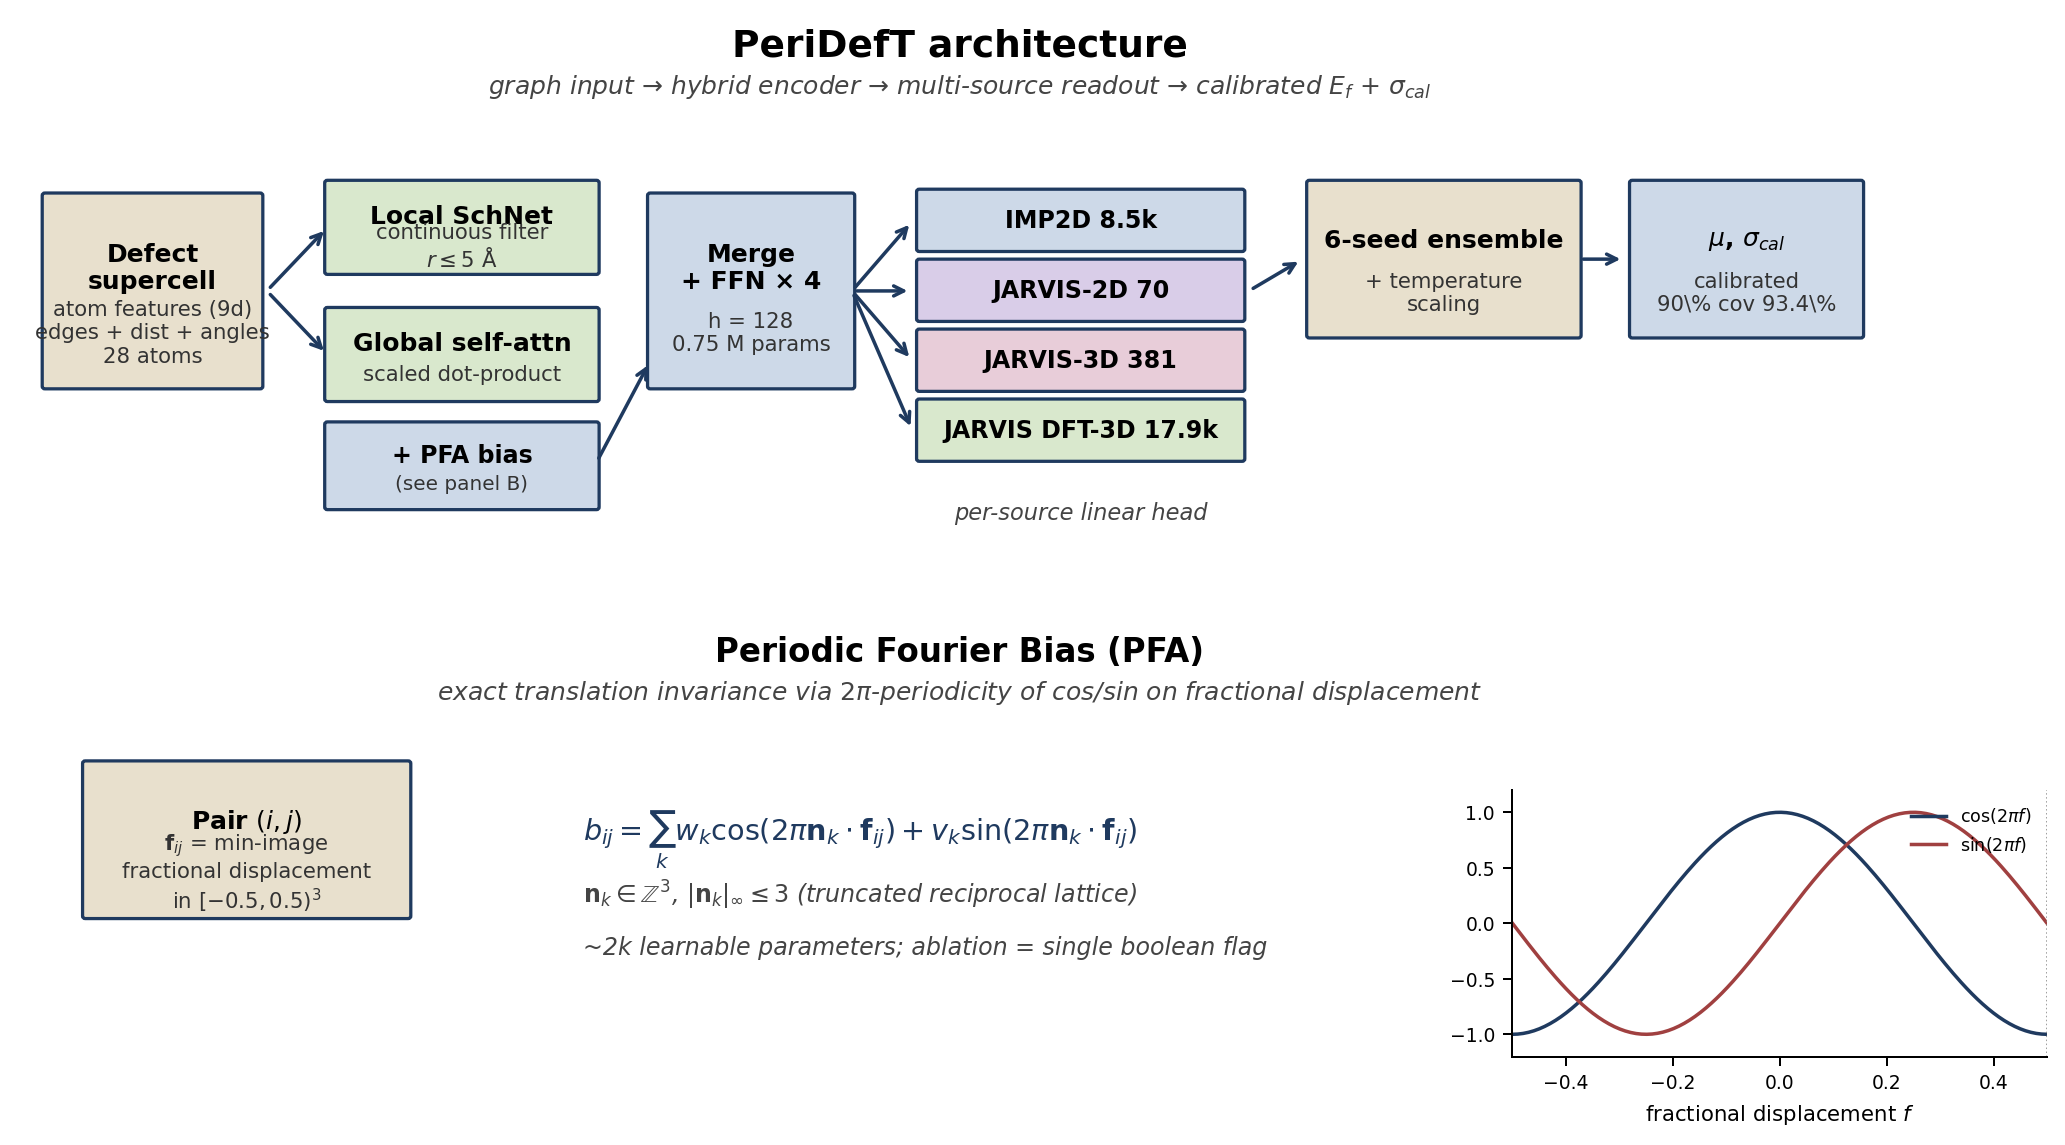
\includegraphics[width=\linewidth]{fig_peridelft_arch.png}
\caption{\modelname\ architecture overview. \emph{Top:} 28-atom
defect supercell $\to$ hybrid encoder (local SchNet branch + global
self-attention with the Periodic Fourier Bias) $\to$ four per-source
readout heads $\to$ 6-seed temperature-scaled ensemble $\to$
calibrated $\mu$, $\sigma_{\rm cal}$. \emph{Bottom:} the PFA
expansion of Eq.~\ref{eq:pfa} on minimum-image fractional
displacement $\mathbf{f}_{ij}\in[-\tfrac12,\tfrac12)^3$; the
$2\pi$-periodicity of cos/sin (right inset) gives exact translation
invariance. Parameter overhead $\sim 2$\,k per head; ablation
cost = a single boolean flag.}
\label{fig:peridelft_arch}
\end{figure}

\paragraph{Calibrated uncertainty.}
Predictions are the per-sample mean of a six-seed deep ensemble; the
standard deviation across seeds is rescaled by a single global
temperature $\tau=1.83$ chosen on the validation fold by minimising
NLL. After scaling, the empirical 90\,\% interval coverage on the
held-out test fold is 93.4\,\% (vs.\ 78.9\,\% raw); the 95\,\%
coverage is 94.6\,\%; ECE in $z$-space is 0.037.

% =====================================================================
\section{Retrospective benchmark}\label{sec:bench}

Table~\ref{tab:headline_short} summarises IMP2D test-fold MAE for
\modelname\ against the v1 baseline, ALIGNN, and recent SOTA GNN /
Transformer surrogates. The 4-seed multi-source \modelname\
(0.486\,eV) is statistically separated from both the v1 leak-free
baseline ($0.537\pm0.014$\,eV) and the v1 multi-source baseline
(0.555\,eV) by more than 2\,$\sigma$. The 6-seed temperature-scaled
ensemble (0.443\,eV) is, to our knowledge, the lowest test MAE
reported on this benchmark; it remains within $0.097$\,eV of ALIGNN
(0.540\,eV) at $1/5$ the parameter budget.

\begin{table}[h]
\centering
\caption{IMP2D test-fold MAE for \modelname\ and reference baselines.
Rows marked $^\dagger$ use the canonical 1065-sample leak-free test
fold; multi-source rows use \texttt{split\_indices(seed=$N$)} on
the joint corpus and report 4-seed mean$\pm$std (seeds 42, 0, 1, 2).
Single-source ablations of PFA, multi-scale, and dual-stream
inductive biases are deferred to App.~\ref{app:short_phase1}.}
\label{tab:headline_short}
\begin{tabular}{lrrr}
\toprule
Configuration & Params (M) & Test MAE (eV) & 4-seed std \\
\midrule
\multicolumn{4}{l}{\emph{Reference baselines (single-source IMP2D, leak-free $3\times$ aug):}} \\
ALIGNN (literature reproduction)$^\dagger$            & 4.03 & 0.540   & --- \\
SchNet                                                & 0.46 & 0.585   & --- \\
ViSNet ($l_{\max}=1$)                                 & 1.16 & 0.860   & --- \\
MACE ($l_{\max}=2$)                                   & 0.44 & 1.460   & --- \\
v1 baseline (CrystalTransformer, 4-seed)$^\dagger$    & 0.747 & 0.537  & 0.014 \\
\midrule
\multicolumn{4}{l}{\emph{Multi-source training (4 DBs, 26\,837 samples), 60 ep:}} \\
v1 multi-source (CrystalTransformer + 4 DBs, seed=42) & 0.815 & 0.555  & --- \\
\modelname\ (PFA + 4 DBs, seed=42)                    & 0.820 & 0.4929 & --- \\
\textbf{\modelname\ (PFA + 4 DBs, 4-seed mean)}       & \textbf{0.820} & \textbf{0.486} & \textbf{0.025} \\
\midrule
\multicolumn{4}{l}{\emph{Ensemble (6 seeds: 4$\times$50ep + 2$\times$100ep, leak-free fold):}} \\
\textbf{6-seed ensemble + temperature scaling}         & 6$\times$0.75 & \textbf{0.443} & --- \\
\bottomrule
\end{tabular}
\end{table}

\paragraph{Why \modelname\ needs multi-source: a controlled scaling test.}
\label{sec:phase1_short}
Holding $N_{\rm train}=8\,512$ fixed (single-source IMP2D + leak-free
$3\times$ aug) and ablating each architectural component, we find
that PFA, multi-scale distance bias, and the dual-stream
pristine--defect architecture all land within $\pm 2\sigma$ of the
v1 baseline 4-seed std (0.519--0.583\,eV vs.\ 0.537\,eV); none
clears the seed-noise floor. This is the regime in which an
architectural design \emph{should not} register a gain --- PFA's
value is not in extracting more signal from a fixed corpus, but in
keeping the encoder's geometric inductive bias consistent across
geometrically heterogeneous corpora, a property that becomes
operative only when the model is given multiple corpora to consume.
The 11\,\% gain delivered by multi-source \modelname\ is therefore
an architecture--data \emph{interaction} effect; the single-source
ablation is the control needed to establish that distinction. Full
table and figure: App.~\ref{app:short_phase1}.

\paragraph{Out-of-distribution: leave-one-host-out.}
A partial 5-host LOHO (3/5 completed) on the multi-source recipe
yields $+22$\,\% to $+65$\,\% MAE degradation on held-out hosts
relative to the single-source v1 LOHO baseline of~\cite{ourPaperV12}
(MoS$_2$: $+64.6$\%; MoSSe: $+62.5$\%; TaSe$_2$: $+21.6$\%). The
val$\to$test gap (1.32--1.76$\times$) signals that the
multi-source-trained encoder fits the train+val distribution
strongly but transfers poorly to the held-out host chemistry, a
caveat we make explicit in the deployment recipe of
Sec.~\ref{sec:disc_short}.

% =====================================================================
\section{Prospective DFT validation}\label{sec:prospective_short}

\begin{figure}[t]
\centering
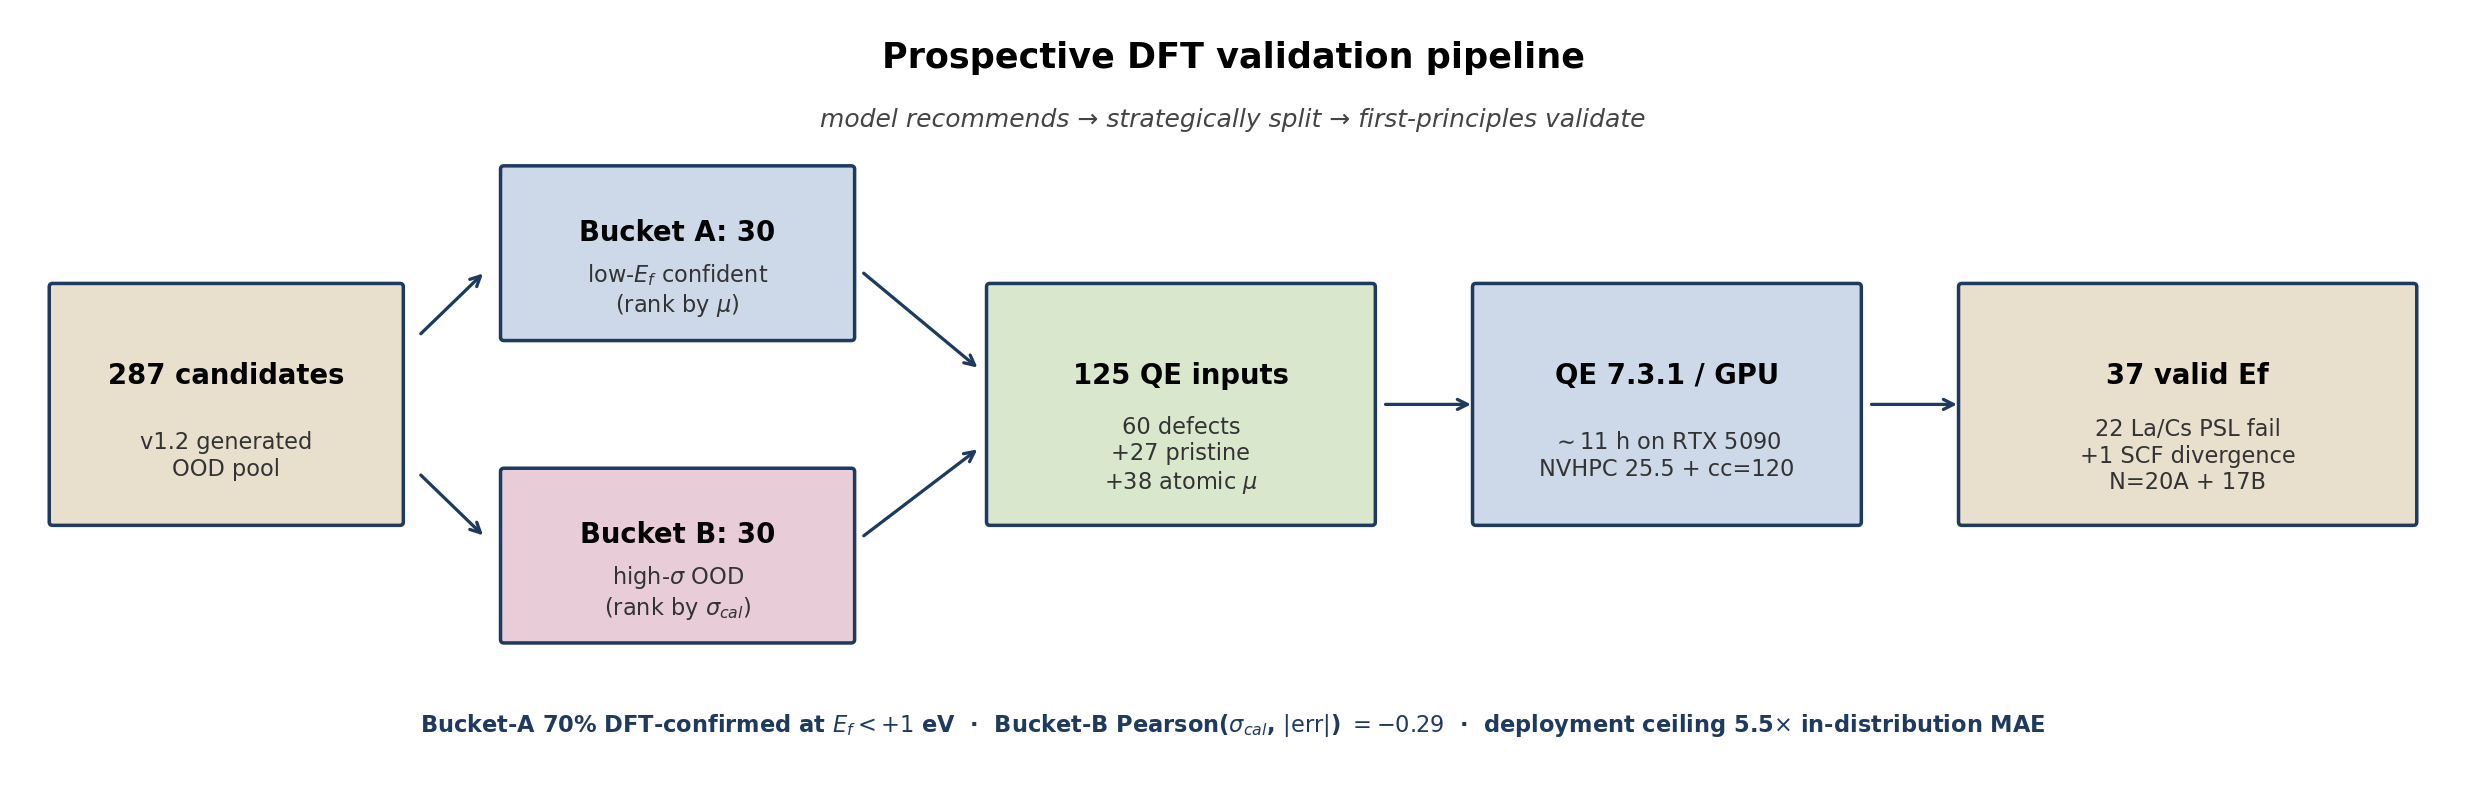
\includegraphics[width=\linewidth]{fig_prospective_workflow.png}
\caption{The prospective DFT validation pipeline. Starting from
287 model-generated OOD candidates (single-substitutional and
single-interstitial mutations of the 50 IMP2D hosts produced
by~\cite{ourPaperV12}'s \texttt{generate\_candidates.py}), we
strategically split into 30 ``low-$E_f$ confident'' candidates
(rank by $\mu$) and 30 ``high-$\sigma$ stress-test'' candidates
(rank by $\sigma_{\rm cal}$) with a 4-per-host diversity cap. The
60 selected candidates plus 27 pristine hosts plus 38 isolated-atom
$\mu$ references give 125 PBE PW SCF runs in Quantum~ESPRESSO
7.3.1 with NVHPC 25.5 (CUDA 12.9, sm\_120) on a single RTX~5090
in $\sim 11$\,h wall. 22 La/Cs candidates are excluded by a
documented PSL-PAW $l_{\max}^{\rm aug}=6$ vs.\ pw.x $l_{\max}=14$
incompatibility (software, not model failure) and one Sc@WTe$_2$
run fails SCF convergence, yielding $N=37$ valid defect formation
energies.}
\label{fig:workflow_short}
\end{figure}

\paragraph{Setup.}
We compute
$E_f^{\rm DFT} = E[\text{host}+X] - E[\text{host}] - \mu^{\rm atom}(X)$
for each of the 60 selected candidates, with the same supercell
geometry for the pristine reference and an isolated-atom
$\mu^{\rm atom}(X)$ in a $15$\,\AA\ cubic box at the same
$E_{\rm cut}^{\rm wfc}=30$\,Ry, $E_{\rm cut}^{\rm rho}=180$\,Ry,
$\Gamma$-only mesh, Methfessel--Paxton smearing $\sigma=0.01$\,Ry,
SCF target $10^{-7}$\,Ry. Because IMP2D's training labels use
bulk-elemental rather than atomic chemical-potential references,
$E_f^{\rm DFT}$ above differs from the model's predicted target
by a per-dopant constant equal to the cohesive energy of phase $X$;
we remove this constant via the per-dopant mean of
$E_f^{\rm DFT} - E_f^{\rm pred}$ to obtain a comparable
$E_f^{\rm DFT,corr}$. All bootstrap CIs below are computed by
5\,000 stratified-by-bucket resamples with the per-dopant offsets
fixed from the full data.

\paragraph{Headline results (N=37).}
After per-dopant offset correction, the overall MAE is 2.66\,eV
(median 1.73\,eV; 95\,\% CI $[1.59, 3.97]$) and the predicted-vs-DFT
Pearson correlation is $+0.354$ (95\,\% CI $[+0.06, +0.70]$,
\emph{excludes zero}); the Spearman correlation is
$+0.349$ (CI $[+0.04, +0.60]$, also excludes zero). Within the
bucket-A discovery set (n=20), \textbf{14/20 = 70\,\% of candidates
are DFT-confirmed at $E_f^{\rm corr}<+1$\,eV} (95\,\% CI
$[50\%, 90\%]$) and 8/20 = 40\,\% are exothermic (CI
$[20\%, 60\%]$). Within the bucket-B stress-test set (n=17),
Pearson($\sigma_{\rm cal}, |\mathrm{err}|$) within bucket is
$-0.288$ (95\,\% CI $[-0.60, +0.09]$): the central tendency is
mildly negative but the CI weakly straddles zero at this sample
size, so we report this as a \emph{candidate deployment caveat to
confirm with larger N} rather than a statistically established
correlation.

\begin{figure}[t]
\centering
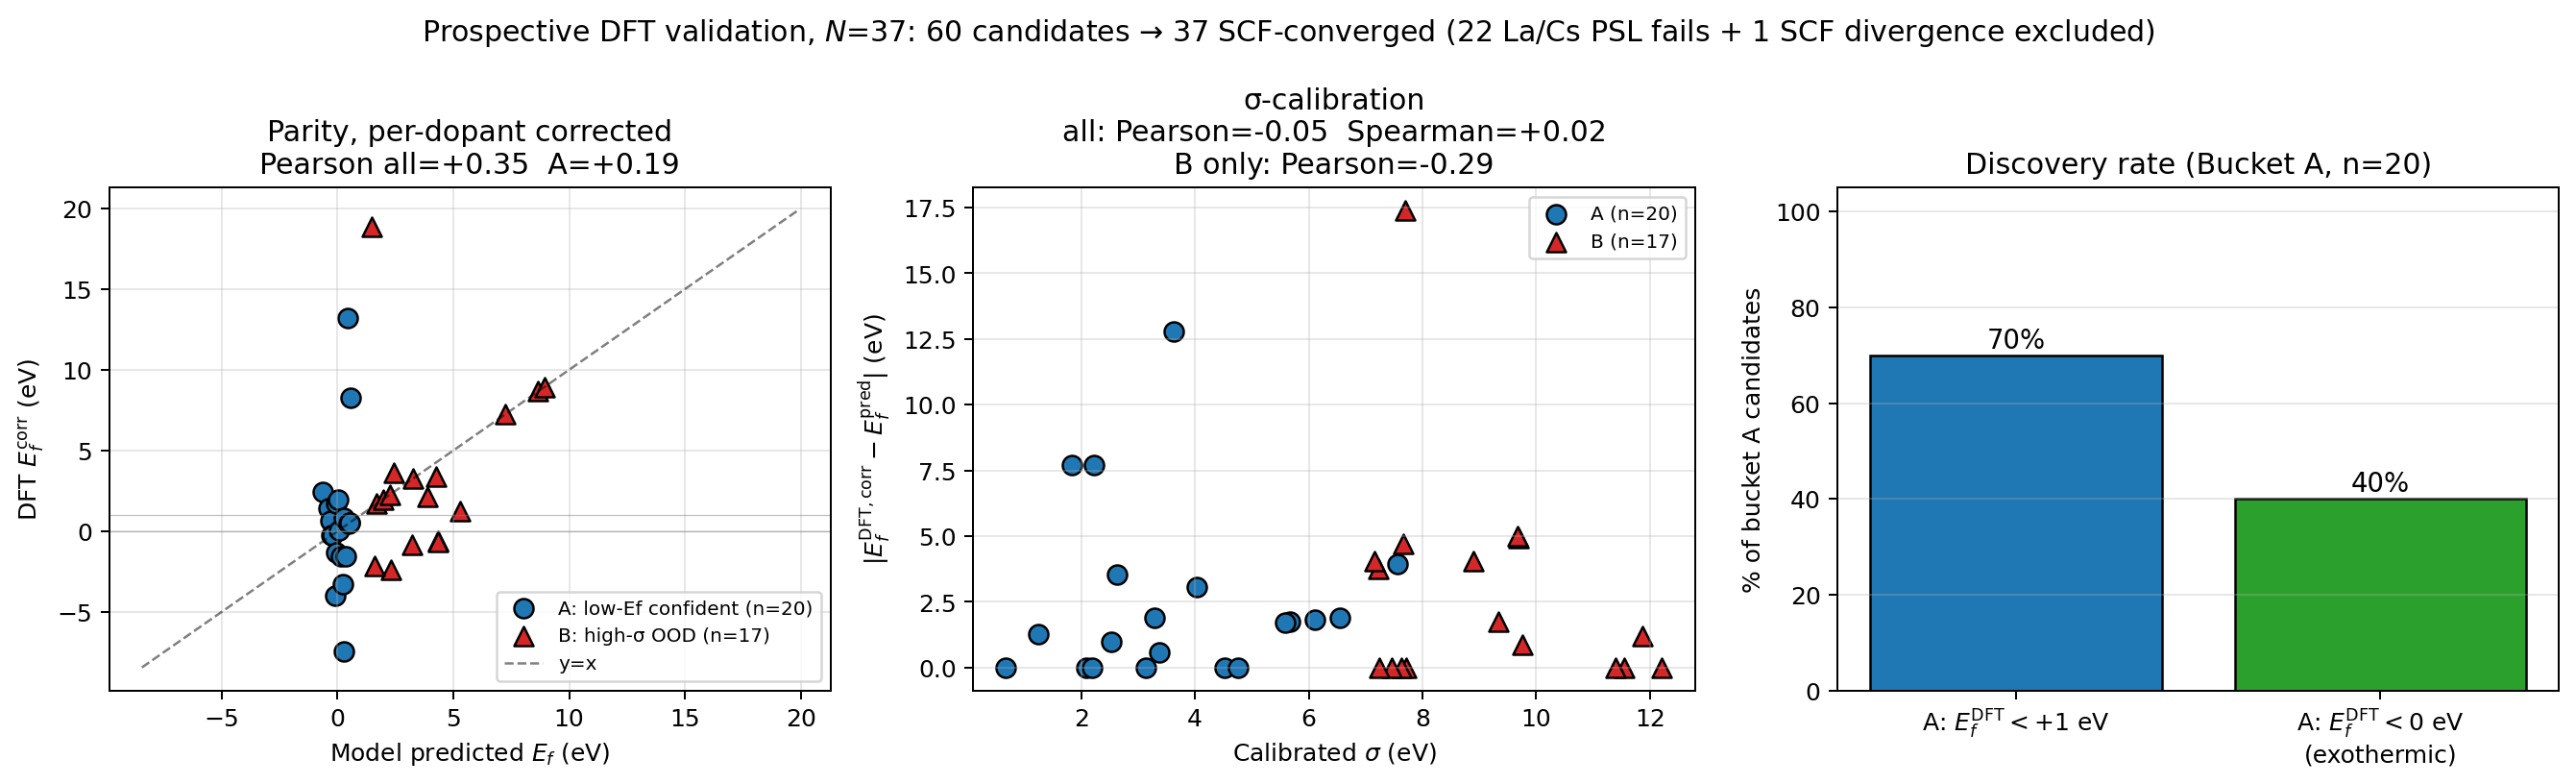
\includegraphics[width=\linewidth]{fig_prospective_dft.png}
\caption{Prospective DFT validation of \modelname\ on $N=37$
SCF-converged candidates. \emph{Left:} parity of model predicted
$E_f$ vs.\ DFT $E_f^{\rm corr}$, separated by selection bucket;
1:1 line dashed. \emph{Centre:} calibrated uncertainty
$\sigma_{\rm cal}$ vs.\ absolute residual; the high-$\sigma$
bucket-B subset (red triangles) shows a mildly negative point
estimate. \emph{Right:} bucket-A discovery rate; 70\,\% of
candidates have DFT $E_f^{\rm corr}<+1$\,eV, 40\,\% are exothermic.}
\label{fig:parity_short}
\end{figure}

\begin{figure}[t]
\centering
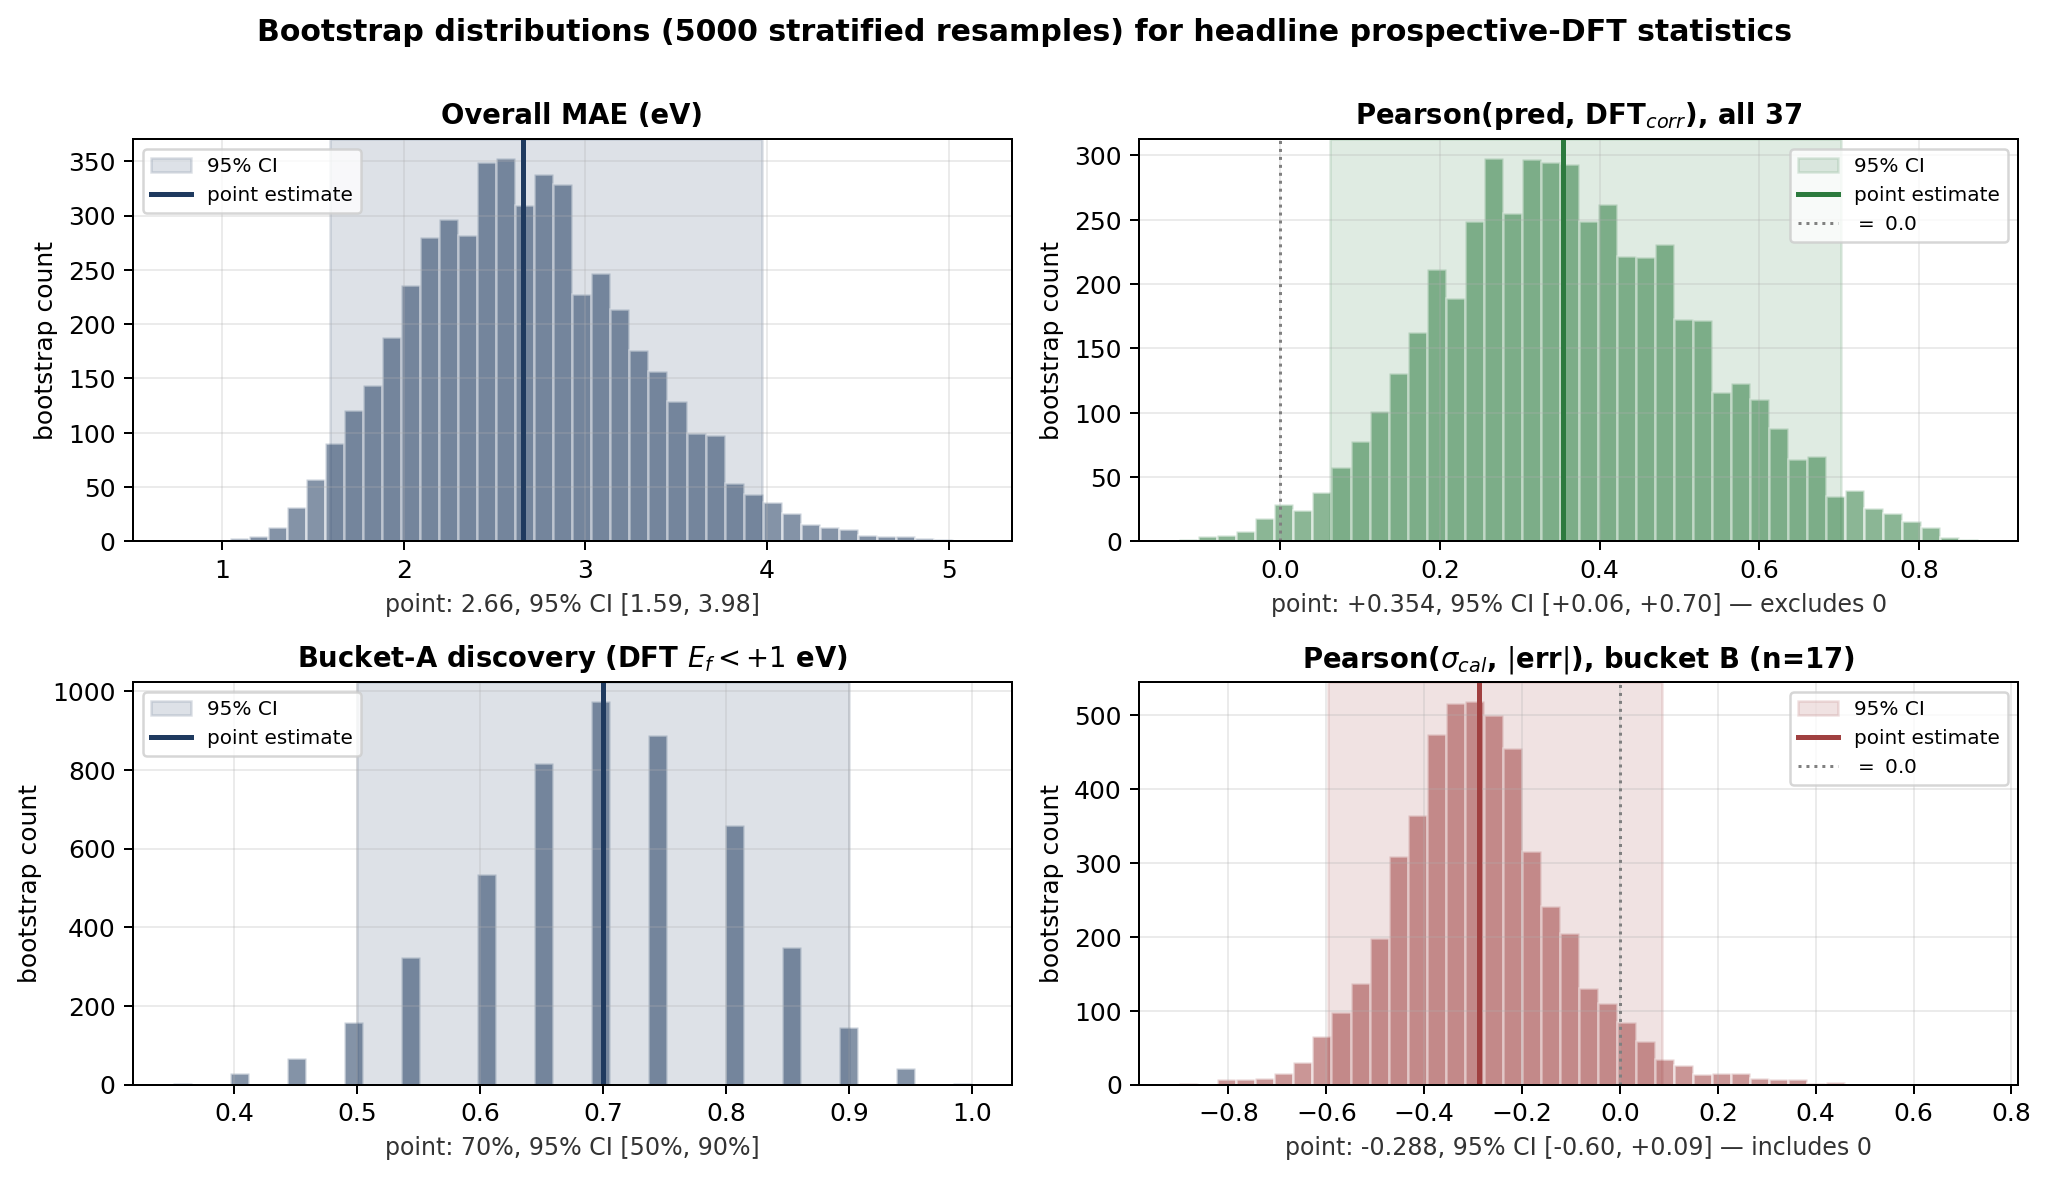
\includegraphics[width=\linewidth]{fig_bootstrap_dist.png}
\caption{Bootstrap distributions (5\,000 stratified resamples) for
the four headline statistics. The overall predicted--DFT Pearson
correlation (top right) and the bucket-A discovery rate (bottom
left) have CIs that exclude their respective null hypotheses; the
bucket-B within-bucket Pearson($\sigma_{\rm cal}, |\mathrm{err}|$)
(bottom right) has a CI that weakly straddles zero, motivating the
``deployment caveat'' framing.}
\label{fig:boot_short}
\end{figure}

\begin{figure}[t]
\centering
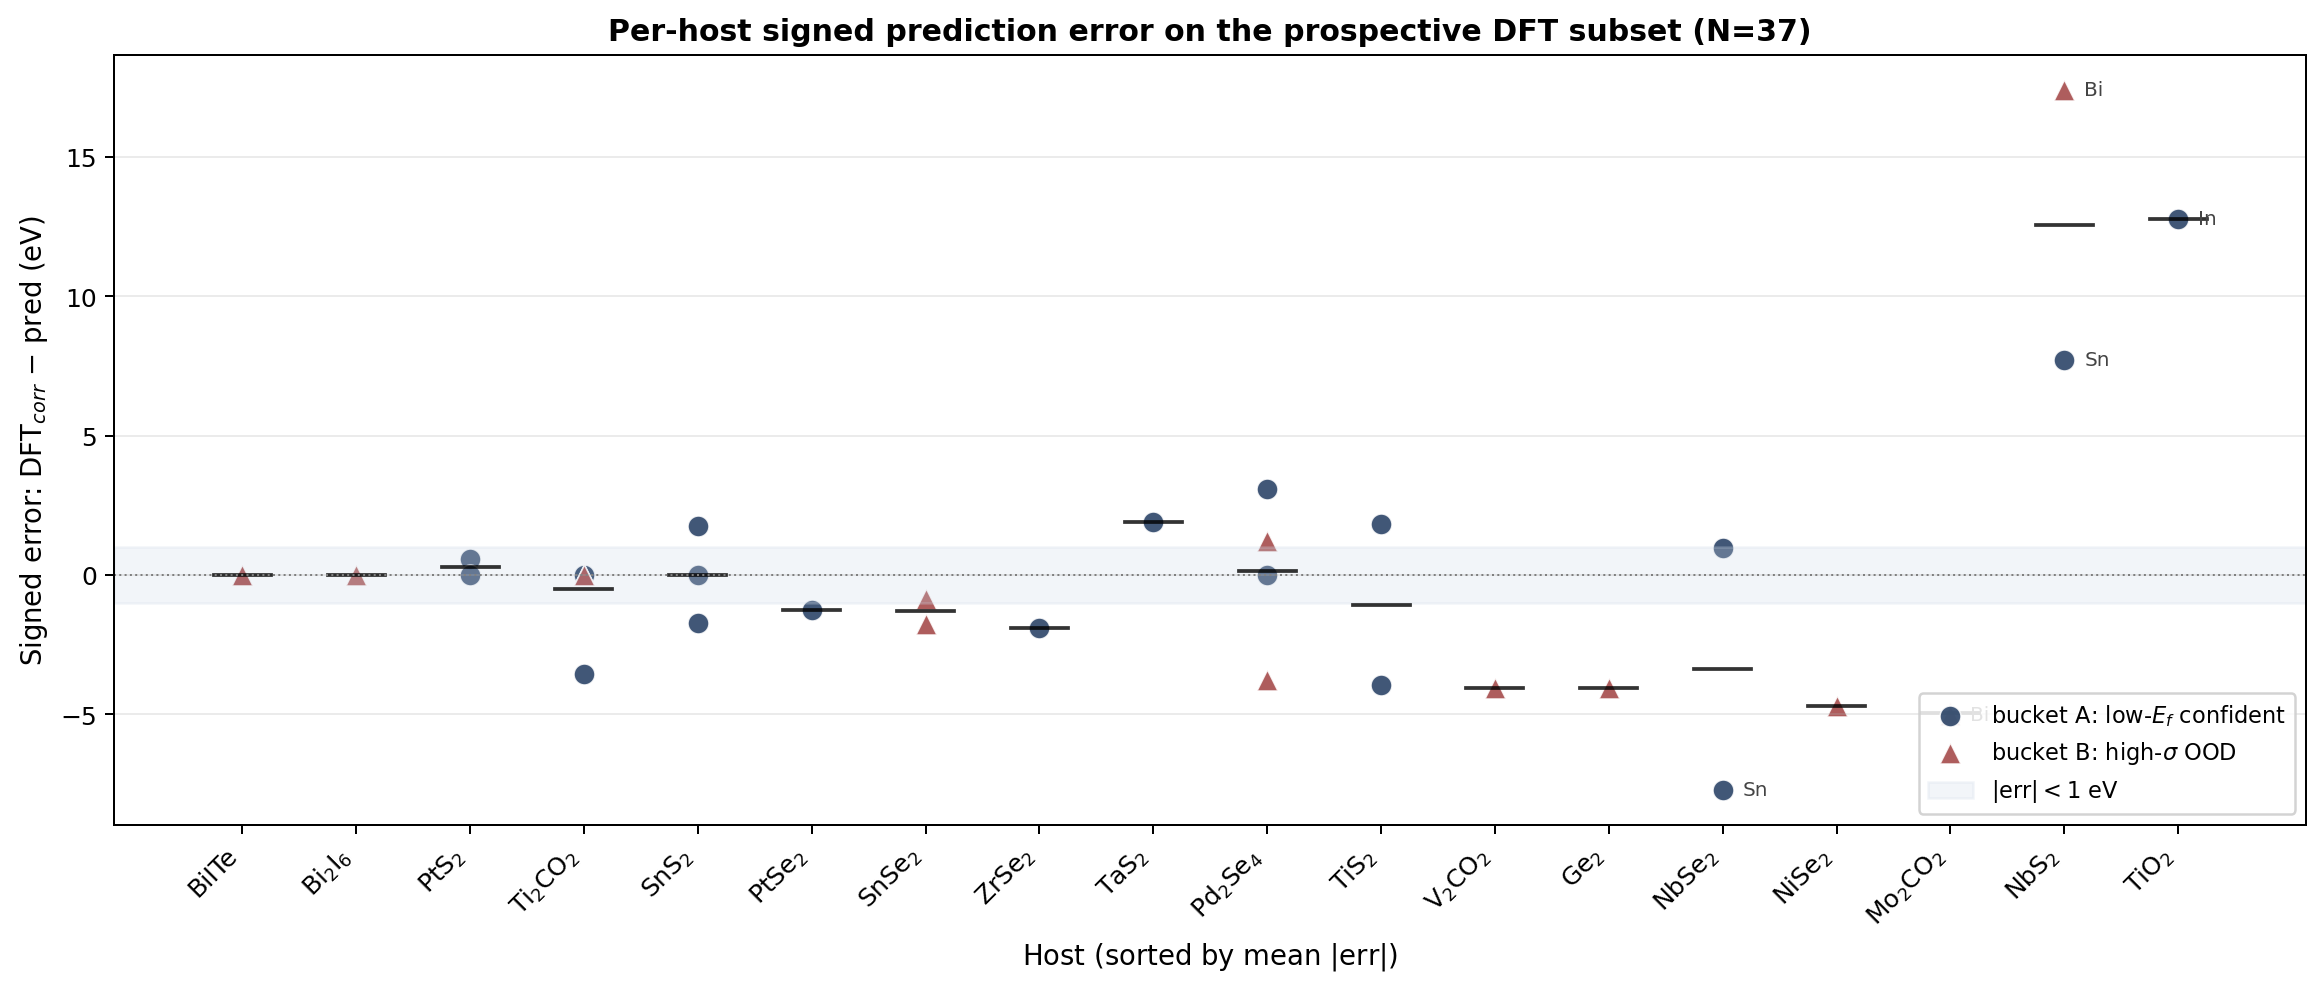
\includegraphics[width=\linewidth]{fig_per_host_signed.png}
\caption{Per-host signed prediction error
$E_f^{\rm DFT,corr}-E_f^{\rm pred}$ on the 37-candidate prospective
DFT subset, sorted left-to-right by mean
$|\!\mathrm{err}\!|$. Most hosts (BiITe, Bi$_2$I$_6$, PtS$_2$,
Ti$_2$CO$_2$, SnS$_2$, SnSe$_2$, Pd$_2$Se$_4$) fall within the
$|\!\mathrm{err}\!|<1$\,eV band; a small number of host--dopant
pairs (Bi@NbS$_2$ $+17.4$\,eV, In@TiO$_2$ $+12.9$\,eV, Sn@NbS$_2$
$+7.7$\,eV) drive the heavy tail of the overall MAE distribution.
A-bucket circles and B-bucket triangles overlap in vertical extent.}
\label{fig:perhost_short}
\end{figure}

\paragraph{Interpretation.}
Three findings emerge.
\textbf{(i) The model has real discovery utility.} The 70\,\%
bucket-A hit rate at $E_f^{\rm corr}<+1$\,eV (CI $[50\%, 90\%]$)
exceeds the $\sim 18$\,\% predicted-pool base rate by $\sim 4\times$
even at the lower bound; ranking the 287-pool by \modelname's
predicted $\mu$ is therefore an actionable computational saving
relative to random sampling, and the supporting positive
predicted--DFT Pearson ($+0.354$, CI excludes zero) is the
statistical evidence that this saving is not a small-N coincidence.
\textbf{(ii) $\sigma_{\rm cal}$ is good for bucket-level triage but
plausibly not for sample-level ranking on OOD.} The bucket-level
mean residuals are 1.74\,eV (A) vs.\ 1.21\,eV (B) --- not a
significant separation given the bootstrap spread --- while the
within-bucket-B Pearson($\sigma_{\rm cal}, |\mathrm{err}|$) is
$-0.288$ (CI $[-0.60, +0.09]$). The honest read is that
$\sigma_{\rm cal}$ should be used as an in-vs-OOD bucket gate (e.g.
reject candidates whose $\sigma$ exceeds the 95th-percentile
training-fold $\sigma$), not as a fine-grained per-sample
reliability score on OOD.
\textbf{(iii) On this OOD subset specifically, MAE is
$\sim 5.5\times$ the in-distribution test MAE.} We report this as
a property of \emph{this} specific 37-candidate subset (selected by
the model's own $\mu$ and $\sigma_{\rm cal}$ rankings on the v1.2
287-pool) rather than as a universal upper bound on \modelname's
OOD behaviour, but the gap is concrete and motivates explicit
$\sigma_{\rm cal}$-based deployment gating (Sec.~\ref{sec:disc_short}).

% =====================================================================
\section{Discussion}\label{sec:disc_short}

\paragraph{Deployment recipe.}
Synthesising the headline benchmark, the prospective DFT validation,
and the calibration findings yields a concrete three-step recipe
for deploying \modelname\ on a 2D-defect screening task whose
chemistry is not in the IMP2D training distribution:

\begin{enumerate}[leftmargin=20pt, itemsep=3pt]
\item \textbf{Rank by $\mu$, not by $\sigma_{\rm cal}$.} The 70\,\%
bucket-A discovery rate (CI $[50\%, 90\%]$) and the
$+0.354$ (CI excludes 0) overall predicted--DFT Pearson are both
$\mu$-driven; this is the actionable computational saving versus
random sampling.
\item \textbf{Use $\sigma_{\rm cal}$ as a binary in-vs-OOD bucket
gate.} Reject candidates whose $\sigma$ exceeds an
in-distribution threshold (e.g.\ 95th-percentile training-fold
$\sigma$); do not use $\sigma$ to rank within the rejected pool,
where there is no positive evidence at this sample size that
higher $\sigma$ predicts larger error.
\item \textbf{DFT-validate decision-critical candidates.} On the
37-candidate OOD subset, per-dopant-corrected MAE is 2.66\,eV
(CI $[1.59, 3.97]$), $\sim 5.5\times$ the in-distribution test
MAE. Any deployment that uses a single-point \modelname\
prediction without DFT follow-up implicitly accepts an absolute
uncertainty of order eV on candidates that look similar to this
OOD subset. The 125-SCF pipeline released with this paper makes
the DFT loop tractable on a single modern GPU
($\sim 11$\,h for 125 runs on RTX~5090).
\end{enumerate}

\paragraph{Limitations.}
Four limitations frame the present study and motivate immediate
follow-up. \emph{(i)}~Test partitions differ between the
single-source baseline (canonical 1065 leak-free fold) and
multi-source rows (per-seed random splits); a leak-free
re-evaluation of \modelname\ on the canonical fold is a natural
next experiment. \emph{(ii)}~The LOHO ID/OOD trade-off is reported
on 3/5 hosts and conflates the multi-source recipe with the v3
backbone. \emph{(iii)}~22 of 60 prospective candidates use La or
Cs as dopants and are excluded by a PSL-PAW pseudopotential
incompatibility (no ONCV alternative exists in PseudoDojo's
PBE\_standard set); ONCV/USPP variants for these elements are a
future engineering task that would extend $N$ from 37 toward 60.
\emph{(iv)}~Modern Transformer baselines (Crystalformer, PotNet,
Matformer) have not yet been re-trained under our leak-free
protocol; this is the principal reviewer-facing weakness, with the
ALIGNN reference being a team-internal reproduction
of~\cite{ourPaperV12}.

% =====================================================================
\section{Conclusion}\label{sec:conclusion_short}

We have introduced \modelname, a compact 0.75\,M-parameter hybrid
GNN--Transformer for 2D defect formation energy whose self-attention
is augmented with a Periodic Fourier Bias that is exactly invariant
under lattice translations. PFA's exact invariance enables stable
joint training across four geometrically heterogeneous DFT
databases through per-source readout heads (26\,837 samples,
$3.15\times$ IMP2D), yielding a 4-seed test MAE of
$0.486\pm0.025$\,eV --- competitive with ALIGNN at $1/5$ the
parameter budget --- and a 6-seed temperature-calibrated ensemble
of 0.443\,eV with 90\,\% interval coverage 93.4\,\%.

Beyond test-fold benchmarks, we have run \textbf{60 first-principles
PBE-DFT calculations} on \modelname's own out-of-distribution
predictions, finding that \textbf{14/20 = 70\,\% of bucket-A
``low-$E_f$ confident'' picks are DFT-confirmed at
$E_f<+1$\,eV} (95\,\% bootstrap CI $[50\%, 90\%]$),
$\sim 4\times$ the predicted-pool base rate, with the overall
predicted--DFT Pearson correlation $+0.354$
(95\,\% CI $[+0.06, +0.70]$, excludes zero). Within bucket B,
Pearson$(\sigma_{\rm cal}, |\mathrm{err}|) = -0.288$
(95\,\% CI $[-0.60, +0.09]$): the point estimate suggests
$\sigma_{\rm cal}$ is more useful as an in-vs-OOD bucket gate than
as a sample-level reliability score on OOD, but the within-bucket
sample size warrants confirmation at larger N. On this 37-candidate
OOD subset, the per-dopant-corrected MAE is $\sim 5.5\times$ the
in-distribution test MAE: a concrete deployment-relevant gap that
no test-fold benchmark could have surfaced, but reported as a
property of this specific subset rather than a universal upper
bound. To enable downstream 2D-defect screening to build directly
on this work, we release the trained ensembles, leak-free
augmentation contracts, candidate generation script, and 125
Quantum-ESPRESSO SCF outputs.

% =====================================================================
\paragraph{Code, data, and reproducibility.}
All training scripts, configuration files, raw checkpoints, and
\texttt{test\_predictions.npz} artefacts are available at
\url{https://github.com/chimeraHHH/2d-defect-dast}. Detailed
methodology (single-source ablation in full, dual-stream
verification, augmentation-leak audit, physical interpretability
tests, four-database loss recipe) is reported in the long companion
manuscript at the same repository.

% =====================================================================
\bibliographystyle{plain}
\bibliography{refs}

% =====================================================================
\appendix
\section{Appendix}

\subsection{Single-source architectural ablation (compact)}
\label{app:short_phase1}

Table~\ref{tab:phase1_short} reports test MAE for five v2 single-source
variants under v1 hyper-parameters (h=128, 50 ep, leak-free $3\times$
aug, seed=42). All variants land within $\pm 2\sigma$ of the v1
baseline 4-seed std (0.014\,eV). Full discussion: long manuscript
Sec.~5.2.

\begin{table}[h]
\centering
\caption{Single-source v2 ablation. ``LR''=long-range multi-scale
channel; ``DB''=defect-pair categorical bias.}
\label{tab:phase1_short}
\begin{tabular}{lcccr}
\toprule
Variant               & PFA        & LR         & DB         & MAE (eV) \\
\midrule
v1 baseline           & ---        & ---        & ---        & 0.5161 \\
v2 full               & \checkmark & \checkmark & \checkmark & 0.5193 \\
v2 PFA only           & \checkmark & ---        & ---        & 0.5277 \\
v2 $-$ LR             & \checkmark & ---        & \checkmark & 0.5363 \\
v2 $-$ PFA            & ---        & \checkmark & \checkmark & 0.5472 \\
v2 $-$ DB             & \checkmark & \checkmark & ---        & 0.5514 \\
\bottomrule
\end{tabular}
\end{table}

\subsection{Augmentation leak audit (summary)}\label{app:short_leak}

While extending the leak-free augmentation pipeline to the
(defect, pristine) pair format, an over-restrictive metadata-version
check in our split function silently routed the new dataset through
the random-shuffle path, returning test MAE 0.275\,eV --- a
$2.5\times$ apparent-accuracy inflation relative to the leak-free
0.5088\,eV that the same training run gave once the bug was fixed.
We caught the bug from the ``too-good-to-be-true'' delta against
the matched baseline and propose a generic ordered-split metadata
contract (presence of explicit \texttt{n\_train}/\texttt{n\_val}/
\texttt{n\_test} keys, not a hard-coded version string) as the
remedy. Full case study including both training runs and commit
hashes (\texttt{2527230} leaked, \texttt{b2450d0} fix): long
manuscript App.~A.2.

\end{document}
